%
% File tupa_multitask.tex

\documentclass[11pt,a4paper]{article}
\usepackage[hyperref]{naaclhlt2018}
\usepackage{times}
\usepackage{latexsym}
\usepackage{tikz}
\usepackage{tikz-dependency}
\usepackage[warn]{textcomp}
\usepackage{subcaption}
\usepackage{multirow}
\usepackage{url}
\usepackage{etoolbox}

\makeatletter
\patchcmd\@combinedblfloats{\box\@outputbox}{\unvbox\@outputbox}{}{%
   \errmessage{\noexpand\@combinedblfloats could not be patched}%
}%
 \makeatother


\usetikzlibrary{shapes,shapes.misc}

%\aclfinalcopy % Uncomment this line for the final submission
%\def\aclpaperid{***} %  Entr the acl Paper ID here

%\setlength\titlebox{5cm}
% You can expand the titlebox if you need extra space
% to show all the authors. Please do not make the titlebox
% smaller than 5cm (the original size); we will check this
% in the camera-ready version and ask you to change it back.

\title{Deep Multitask Learning for Transition-Based DAG Parsing}

\author{Daniel Hershcovich$^{1,2}$ \\
  \\\And
  Omri Abend$^2$ \\
  $^1$The Edmond and Lily Safra Center for Brain Sciences \\
  $^2$School of Computer Science and Engineering \\
  Hebrew University of Jerusalem \\
  \texttt{\{danielh,oabend,arir\}@cs.huji.ac.il}
  \\\And
  Ari Rappoport$^2$
}

\date{}

\begin{document}
\maketitle
\begin{abstract}
  We train a transition-based DAG parser on multiple semantic parsing tasks.
  In a multitask setting, we observe improvements on a low-resource task,
  Universal Conceptual Cognitive Annotation parsing, using other schemes
  as auxiliary tasks.
  Despite various divergences between semantic representation schemes,
  there are many commonalities both structurally and in terms of semantic content.
  We convert these schemes into a unified format and investigate how
  the similarity between different tasks is related to the contribution of
  using one as an auxiliary task for another.
  Given similar tasks, a BiLSTM-based neural network is able to generalize
  using a shared representation, and effectively gains more training data
  for the low-resource task.
\end{abstract}

\section{Introduction}\label{sec:introduction}

While the development of syntactic treebanks has had a tremendous impact on natural language processing,
semantic representation has arguably yet to reach its full potential in terms of its contribution
to downstream linguistic tasks.
As an example for syntactic annotation, the Universal Dependencies (UD) project provides
cross-linguistically consistent treebanks in many languages \cite{nivre2016universal},
and accurate parsers based upon it and other datasets have been extremely useful in natural
language understanding tasks \cite{P16-1139,E17-1117,K17-3002}.
Semantic representation, while increasingly adopting whole-text annotation rather than more specific
shallow schemes, faces several challenges: semantic distinctions, besides requiring deeper understanding
and being harder to learn, are not always well-defined, and progress is hindered by fragmentation.
Semantic schemes diverge in the content they choose to annotate, their coupling with syntax,
and their degree of cross-linguistic applicability and consistency \cite{abend2017state}.

Recent developments in semantic parsing have targeted, among others,
Abstract Meaning Representation \cite[AMR;][]{banarescu2013abstract,damonte-17,11099},
bilexical Semantic Dependencies \cite[SDP;][]{oepen2014semeval,oepen2015semeval,oepen2016towards,P17-1186}
with target representations such as DELPH-IN MRS \cite[DM;][]{flickinger2012deepbank},
and Universal Conceptual Cognitive Annotation \cite[UCCA;][]{abend2013universal,hershcovich2017a}.
Although each of these tasks has a different graph structure in general,
they are all concerned with whole-sentence (or whole-paragraph) semantic analysis,
and due to the structure of phenomena such as predicate-argument relations,
require parsers that can handle non-projectivity (or discontinuity) and reentrancy, resulting in
directed acyclic graphs (DAGs).
While each of these schemes also focuses on a different set of distinctions,
much of the semantic content is shared.

In cases where related tasks can be learned jointly,
deep multitask learning models have been shown to be successful in various fields of NLP
\cite{collobert2008unified,Zhang2016StackpropagationIR,P17-1186,swayamdipta2017frame,guo2016exploiting}.
We build on these ideas and propose a transition-based semantic DAG parser for UCCA,
trained in a multitask setting to obtain state-of-the-art results.\footnote{Our code is publicly available at ***}


\begin{figure*}
\begin{subfigure}[t]{0.5\textwidth}
  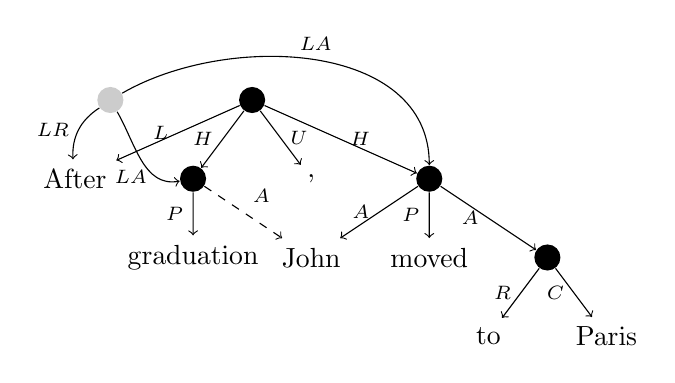
\begin{tikzpicture}[level distance=10mm, ->]
    \node (ROOT) [fill=black, circle] {}
      child {node (After) {After} edge from parent node[left] {\scriptsize $L$}}
      child {node (graduation) [fill=black, circle] {}
      {
        child {node {graduation} edge from parent node[left] {\scriptsize $P$}}
      } edge from parent node[left] {\scriptsize $H$} }
      child {node {,} edge from parent node[right] {\scriptsize $U$}}
      child {node (moved) [fill=black, circle] {}
      {
        child {node (John) {John} edge from parent node[left] {\scriptsize $A$}}
        child {node {moved} edge from parent node[left] {\scriptsize $P$}}
        child {node [fill=black, circle] {}
        {
          child {node {to} edge from parent node[left] {\scriptsize $R$}}
          child {node {Paris} edge from parent node[left] {\scriptsize $C$}}
        } edge from parent node[left] {\scriptsize $A$} }
      } edge from parent node[right] {\scriptsize $H$} }
      ;
    \draw[dashed,->] (graduation) to node [auto] {\scriptsize $A$} (John);
    \node (LKG) at (-1.8,0) [fill=black!20, circle] {};
    \draw[bend right] (LKG) to node [auto, left] {\scriptsize $LR$} (After);
    \draw (LKG) to[out=-60, in=190] node [below] {\scriptsize $LA\quad$} (graduation);
    \draw (LKG) to[out=30, in=90] node [above] {\scriptsize $LA$} (moved);
  \end{tikzpicture}
  \caption{UCCA graph.
  The dashed edge is remote.
  The gray node and its outgoing edges represent linkage between the two scenes.
  Pre-terminal nodes and edges are omitted for brevity.}
  \label{fig:original_example_ucca}
\end{subfigure}
~
\begin{subfigure}[t]{0.5\textwidth}
  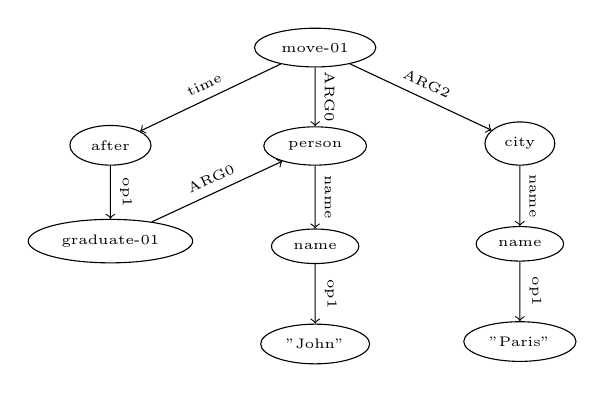
\begin{tikzpicture}[level distance=15mm, ->,
      every node/.append style={sloped,anchor=south,auto=false,font=\tiny},
      level 1/.style={sibling distance=26mm}]
    \node (ROOT) [draw=black,ellipse] {move-01}
      child {node [draw=black,ellipse] {after}
      {
            child {node (graduation) [draw=black,ellipse] {graduate-01} edge from parent node {op1} }
      } edge from parent node {time} }
      child {node (John) [draw=black,ellipse] {person}
      {
        child {node [draw=black,ellipse] {name}
        {
            child {node [draw=black,ellipse] {"John"} edge from parent node {op1} }
        } edge from parent node {name} }
      } edge from parent node {ARG0} }
      child {node [draw=black,ellipse] {city}
      {
        child {node [draw=black,ellipse] {name}
        {
            child {node [draw=black,ellipse] {"Paris"} edge from parent node {op1} }
        } edge from parent node {name} }
      } edge from parent node {ARG2} }
      ;
      \draw (graduation) to node {ARG0} (John);
  \end{tikzpicture}
  \captionof{figure}{AMR graph.
  The text tokens are not part of the graph, and must be matched to
  concepts and constants by alignment.
  Variables are represented by their concepts.}
  \label{fig:original_example_amr}
\end{subfigure}

\begin{subfigure}[t]{0.5\textwidth}
    \begin{dependency}[text only label, label style={above}, font=\small]
    \begin{deptext}[column sep=1em,ampersand replacement=\^]
    After \^ graduation \^ , \^ John \^ moved \^ to \^ Paris \\
    \end{deptext}
        \depedge{1}{2}{ARG2}
        \depedge{5}{4}{ARG1}
        \depedge[edge unit distance=2ex]{1}{5}{ARG1}
        \deproot{5}{top}
        \depedge[edge unit distance=4ex, edge start x offset=-1ex]{5}{7}{ARG2}
        \depedge[edge start x offset=1ex]{6}{5}{ARG1}
        \depedge{6}{7}{ARG2}
    \end{dependency}
  \captionof{figure}{SDP graph (in the DM formalism).
  The graph contains multiple roots: ``After'', ``moved'' and ``to''.
  One of the roots is marked as \textit{top}: ``moved''.
  Punctuation is not included in the graph as it is non-content-bearing.}
  \label{fig:original_example_sdp}
\end{subfigure}
~
\begin{subfigure}[t]{0.5\textwidth}
    \begin{dependency}[text only label, label style={above}, font=\small]
    \begin{deptext}[column sep=1em,ampersand replacement=\^]
    After \^ graduation \^ , \^ John \^ moved \^ to \^ Paris \\
    \end{deptext}
        \depedge{2}{1}{case}
        \depedge{4}{3}{punct}
        \depedge{5}{4}{nsubj}
        \depedge{2}{5}{obl}
        \depedge{7}{6}{case}
        \deproot{5}{root}
        \depedge{5}{7}{obl}
    \end{dependency}
  \captionof{figure}{UD tree.
  Each word has exactly one head, and there is a single root.
  Edge labels correspond to syntactic relations.}
  \label{fig:original_example_ud}
\end{subfigure}

\caption{Example graph in each target representation.}
\label{fig:original_examples}
\end{figure*}

\section{Tasks}\label{sec:tasks}

In this work, we focus on representation schemes providing a \textit{whole-sentence} analysis,
that is, annotating a graph connecting all (content) words in a sentence (or a piece of text in general).
This is in contrast to ``shallow'' semantic parsing,
such as Semantic Role Labeling
\cite[SRL;][]{Palmer:05,gildea2002automatic,swayamdipta2017frame,ringgaard2017sling},
or parsing to logical forms.
We consider four target representations: UCCA, AMR, DM and UD.
Figure~\ref{fig:original_examples} shows an example graph for each scheme,
annotating the sentence ``After graduation, John moved to Paris''.

\subsection{Universal Conceptual Cognitive Annotation}\label{sec:ucca}

UCCA \cite{abend2013universal} is a semantic representation scheme whose main principles
are ease of annotation and cross-linguistic applicability and stability.

UCCA represents the semantics of natural language utterances
as directed acyclic graphs (DAGs), where terminal nodes (nodes without children)
correspond to the text tokens, and
non-terminal nodes to semantic or cognitive entities or relations.
Edges are labeled, indicating the role of a child in the relation the parent represents.
Nodes and edges may belong to one of several \textit{layers}, each corresponding
to a ``module'' of semantic distinctions.
UCCA's \textit{foundational layer} mostly covers predicate-argument
structure, coordination and multi-word expressions.
The \textit{linkage} layer covers relations between events, including temporal and discourse relations
(exemplified by the gray node and its outgoing edges in Figure~\ref{fig:original_example_ucca}).

UCCA's guidelines distinguish between \textit{primary} edges, corresponding to the roles explicit
in the text, and \textit{remote} edges (such as the dashed edge in
Figure~\ref{fig:original_example_ucca}), corresponding to implicit relations.
Primary edges form a tree structure in each layer,
whereas the remote edges enable reentrancy (a DAG structure).

Given UCCA's currently small corpus size (see \S\ref{sec:data}), we hypothesize it will benefit
from multitask learning. We therefore focus on UCCA parsing evaluation---specifically, on the
foundational layer.


\subsection{Abstract Meaning Representation}\label{sec:amr}

AMR \cite{banarescu2013abstract}
is a semantic representation that embeds annotations related
to named entity recognition, semantic role labeling, word
sense disambiguation and co-reference resolution.
AMRs are rooted and directed graphs, in which both nodes and edges are labeled.
Most AMRs are DAGs, although cycles are permitted.
AMR was targeted in the SemEval 2017 shared task \cite{may2017semeval}.

As can be seen in Figure~\ref{fig:original_example_amr}, text tokens are not part
of the AMR graph, which connects only variables, concepts (from a pre-defined set)
and constants (which may be strings or numbers).
During the process of parsing from plain text to AMR,
the tokens are aligned to graph nodes,
a process referred to as \textit{concept identification}.
We use AMR datasets containing already automatically aligned graphs.

\subsection{Semantic Dependency Parsing}\label{sec:sdp}

SDP \cite{oepen2014semeval,oepen2015semeval,oepen2016towards}
is a set of related tasks, targeted in two SemEval shared tasks.
They correspond to four semantic representation schemes, referred to as
DM, PAS, PSD and CCD, representing
predicate-argument relations between content-bearing words in a sentence.
All are based on semantic formalisms whose annotations have been
converted into bilexical dependencies, that is,
labeled directed graphs whose nodes are all text tokens and each edge connects two of them.
Edges are labeled, encoding semantic relations between the tokens.
Non-content-bearing tokens, such as punctuation,
may be left out of the analysis (see Figure~\ref{fig:original_example_sdp}),
but the subgraph restricted to content-bearing tokens is connected.
Graphs containing cycles have been removed from the SDP datasets.

We consider one of the three formalisms used in the SemEval shared task:
the DM (DELPH-IN MRS) representation, which comes
from DeepBank \cite{flickinger2012deepbank},
manually-corrected parses from the LinGO
English Resource Grammar \cite{copestake2000open}.
LinGO is a head-driven phrase
structure grammar \cite[HPSG; ][]{pollard1994head}
with minimal recursion semantics \cite{copestake2005minimal}.

\subsection{Universal Dependencies}\label{sec:ud}

UD \cite{nivre2016universal,11234/1-2515} has become
the dominant dependency representation for
annotating treebanks in a large variety of languages,
aiming for cross-linguistically consistent treebank
annotations for as many languages as possible.
Representations are bilexical trees, with edge labels representing
syntactic relations between the text tokens.

Although not a semantic representation scheme,
we use UD as an auxiliary task,
inspired by recent work showing benefit from using syntax as an auxiliary task for semantic role labeling
\cite[syntactic scaffolding; ][]{swayamdipta2017frame}.
While our main experiments are on English,
thanks to UD's annotation in multiple languages, we can use it as an auxiliary task
for UCCA parsing in German and French, too (see \S\ref{sec:multilingual}).

In addition the basic UD trees (such as in Figure~\ref{fig:original_example_ud}),
\textit{enhanced} and \textit{enhanced++} UD graphs are available for English,
using automatic converters included in Stanford CoreNLP \cite{SCHUSTER16.779}.
These include additional and augmented relations between content words,
partially overlapping with the notion of remote edges in UCCA.
We use the enhanced++ UD representation in our English experiments.



\section{Transition-based universal parser}\label{sec:model}

All target representations introduced in \S\ref{sec:tasks} exhibit
reentrancy and discontinuity (non-projectivity), to varying degrees.
In addition, UCCA and AMR contain non-terminal nodes.
To parse graphs with these structural properties,
we extend TUPA \cite{hershcovich2017a},
a transition-based parser that supports them,
originally developed for UCCA parsing.
TUPA's general transition system allows parsing any DAG structure with labeled edges,
whose terminals are aligned to text tokens.
To support AMR parsing, we take advantage of automatic alignments during training
(\S\ref{sec:conversion}).

Transition-based parsers \cite{Nivre03anefficient} apply \textit{transitions}
incrementally to an internal state defined by
a buffer $B$ of remaining tokens and nodes,
a stack $S$ of incomplete nodes,
and a labeled graph $G$ of constructed nodes and edges.
When the parsing process is finished, the graph $G$ is the final output.
A classifier is used at each step to select the next transition based on features
encoding the current state.
During training, an oracle creates training instances for the classifier,
based on gold-standard annotations.


\subsection{Transition set}\label{sec:transition_set}
Given a sequence of tokens $w_1, \ldots, w_n$,
we predict a rooted graph $G$ whose terminals are the tokens.
Parsing starts with the root node on the stack,
and the input tokens in the buffer.

The TUPA transition set includes
the standard \textsc{Shift} and \textsc{Reduce} operations,
\textsc{Node$_X$} for creating a new non-terminal node and an $X$-labeled edge,
\textsc{Left-Edge$_X$} and \textsc{Right-Edge$_X$} to create a new primary $X$-labeled edge,
\textsc{Left-Remote$_X$} and \textsc{Right-Remote$_X$} to create a new remote $X$-labeled edge,
\textsc{Swap} to handle discontinuous nodes,
and \textsc{Finish} to mark the state as terminal.

Although UCCA contains nodes without any text tokens as descendants
(these nodes are referred to as \textit{implicit units}),
the standard evaluation for UCCA \cite{abend2013universal} is span-based and
ignores these nodes.
For this reason we follow \citet{hershcovich2017a} and do not include
any transition to create these when parsing UCCA,
thus ignoring them in both training and evaluation.
This phenomenon is even more common in AMR, as any unaligned concept
will correspond to implicit nodes.
These may result from alignment errors,
or from abstract concepts,
which have no explicit grounding in the text \cite{buys2017oxford}.
The TUPA transition set does not support node labels either, as only edges are labeled in UCCA.
In AMR, however, node labels correspond to concepts and constants.
When training on AMR, we will ignore any implicit nodes, and produce graphs with only edge labels.
In training, though, we can still use gold node labels for feature extraction.

\subsection{Classifier}\label{sec:classifier}
To select the next transition at each time step,
we use a bidirectional LSTM with embeddings as inputs,
followed by a feedforward network and a softmax layer for classification (see
Figure~\ref{fig:single_model}).
Inference is performed greedily,
and training is done with an oracle that provides the set of all correct transitions at a given state.
The network is trained to maximize the log-likelihood of all correct transitions at
each step, and the actual transition taken in training is the correct transition
with the highest score given by the classifier.

\begin{figure}[t]
   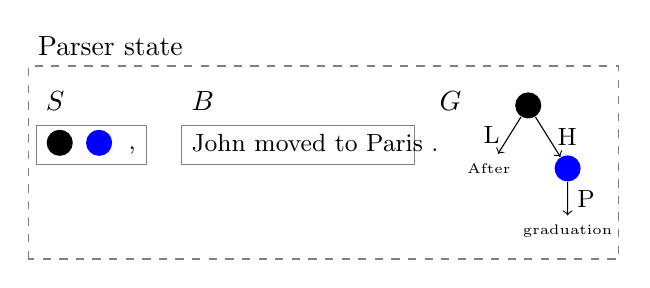
\begin{tikzpicture}[level distance=8mm, sibling distance=1cm]
   \node[anchor=west] at (0,1.5) {Parser state};
   \draw[color=gray,dashed] (0,-1.2) rectangle (7.5,1.25);
   \draw[color=gray] (.1,0) rectangle (1.5,.5);
   \node[anchor=west] at (.1,.8) {$S$};
   \node[fill=black, circle] at (.4,.275) {};
   \node[fill=blue, circle] at (.9,.275) {};
   \node[anchor=west] at (1.15,.175) {\small ,};
   \draw[color=gray] (1.95,0) rectangle (4.9,.5);
   \node[anchor=west] at (1.95,.8) {$B$};
   \node[anchor=west] at (1.95,.275) {\small John moved to Paris .};
   \node[anchor=west] at (5.1,.8) {$G$};
   \node[fill=black, circle] at (6.35,.75) {}
     child {node  {\tiny After} edge from parent [->] node[left] {\small L}}
     child {node [fill=blue, circle] {}
     {
       child {node {\tiny graduation} edge from parent [->] node[right] {\small P}}
     } edge from parent [->] node[right] {\small H} };
   \end{tikzpicture}
   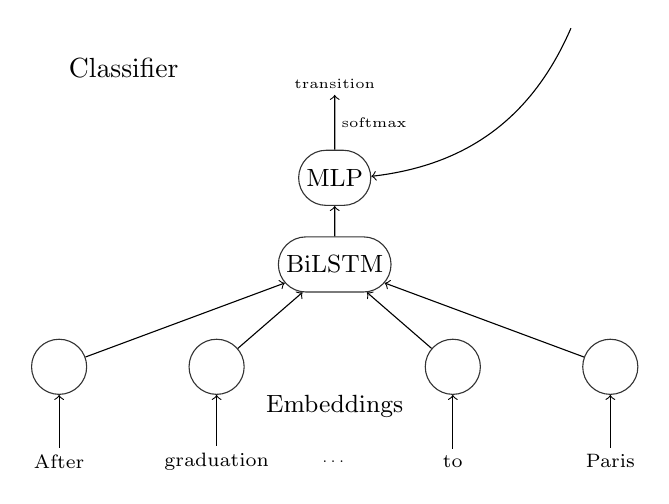
\begin{tikzpicture}[->]
   \node[anchor=west] at (0,6) {Classifier};
   \tiny
   \tikzstyle{main}=[rounded rectangle, minimum size=7mm, draw=black!80, node distance=12mm]
   \node[main] (specific) at (3.5,3.5) {\small BiLSTM};
   \node (embeddings) at (3.5,1.7) {\small Embeddings};
   \foreach \i/\word in {0/{After},2/{graduation},5/{to},7/{Paris}} {
       \node (x\i) at (\i,1) {\scriptsize \word};
       \node[main] (e\i) at (\i,2.2) {};
       \path (x\i) edge (e\i);
       \path (e\i) edge (specific);
   }
    \node (x4) at (3.5,1) {\ldots};
    \node[main] (mlp) at (3.5,4.6) {\small MLP};
    \path (specific) edge (mlp);
    \coordinate (state) at (6.5,6.5);
    \path (state) edge [bend left] (mlp);
    \node (transition) at (3.5,5.8) {transition};
    \path (mlp) edge node[right] {softmax} (transition);
   \end{tikzpicture}
	\caption{Illustration of the TUPA model, adapted (with permission) from \citet{hershcovich2017a}.
		Top: parser state.
		Bottom: BiLTSM architecture.}
	\label{fig:single_model}
\end{figure}

\paragraph{Features.}
In addition to the features used by \citet{hershcovich2017a},
representing the words, POS tags, syntactic dependency relations, and previously predicted edge labels
for nodes in specific locations in the parser state,
we use feature embeddings representing lemmas, word prefixes, suffixes and shapes, and named entities.
For AMR we add node label features according to gold node labels.

\paragraph{Training.}
Features are extracted using spaCy \cite{spacy2}.\footnote{\url{https://spacy.io}}
All embeddings are initialized randomly.
For words, we additionally use external word embeddings containing 250K word vectors from fastText
\cite{bojanowski2016enriching}, pre-trained over Wikipedia and updated during training.
We use dropout \cite{srivastava2014dropout} between MLP layers and recurrent dropout
\cite{NIPS2016_6241} between BiLSTM layers, both with a probability of 0.4.
In addition, we use word, tag and dependency relation dropout:
with a probability of $\frac{0.2}{\#(w)+0.2}$, the embedding is replaced with a zero vector.
For optimization we a minibatch size of 100, decaying all weights by $10^{-5}$ at each update,
and train with stochastic gradient descent (SGD) for 40 epochs with a learning
rate of 0.1, followed by AMSGrad \cite{j.2018on} for 60 epochs with
$\alpha=0.001,\beta_1=0.9,\beta_2=0.999$.
We select the epoch with the best labeled F1 score on the development set.
The neural network is implemented using DyNet \cite{neubig2017dynet}.\footnote{\url{https://dynet.io}}
Hyperparameter settings are listed in Table~\ref{tab:hyperparams}.

\paragraph{Ensembling.}
During inference, we use three models trained with different random seeds, and use
Product of Experts \cite[PoE; ][]{hinton2002training} to combine their predictions:
score vectors after $\log(\mathrm{softmax})$) are added, and the highest-scoring transition
according to the result is selected.

\begin{table}
\begin{tabular}{l|ccccc}
\hline
\footnotesize Dimensions &  main & aux & shared \\
\hline
external word &&& 300 \\
word &&& 200 \\
POS tag &&& 20 \\
syntactic dep. &&& 10 \\
named entity &&& 3 \\
punctuation & & & 1 \\
action & & & 3 \\
node label (AMR) & & 20 \\
edge label & 20 & 20 \\
MLP \#layers & 2 & 1 \\
MLP layer dim. & 50 & 50 \\
BiLSTM \#layers & 2 & 1 & 2 \\
BiLSTM layer dim. & 250 & 50 & 250
\end{tabular}
\caption{Hyperparameter settings.\label{tab:hyperparams}}
\end{table}


\subsection{Constraints}

As each annotation scheme has different constraints on the allowed graphs,
we defined these constraints separately for each task.
During training and parsing, the constraint set corresponding to the task is
selected and applied to the parser state.

Some constraints are task-specific, while some are generic.
For example, in UCCA, a terminal may only have one parent.
In AMR, a concept corresponding to a PropBank frame may have only core arguments defined for the frame.

As an example for a generic constraint, nodes that have already been swapped
should never be swapped again.
To implement this constraint efficiently, we define a \textit{swap index}
for each node, which is assigned when the node is created.
At parse start, only the root node and terminals exist.
We assign the root a swap index of 0, and for each terminal, its swap index
is its position in the text (starting at 1).
Whenever a node is created as a result of a \textsc{Node}
transition, we assign its swap index to be the arithmetic mean of the stack top and buffer
head's swap indices.


\subsection{Unlabeled parsing}\label{sec:unlabeled}

We extend the parser to support unlabeled parsing by simply removing all labels from
\textsc{Edge}, \textsc{Remote} and \textsc{Node} transitions output by the oracle.
This results in a much smaller output dimension, but of course only unlabeled evaluation is
meaningful in this case.


\begin{figure*}[t]
\begin{subfigure}{0.5\textwidth}
    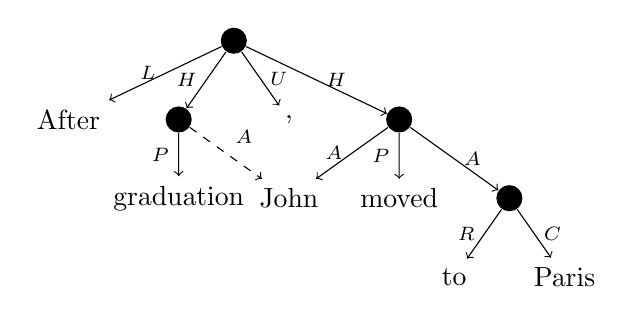
\begin{tikzpicture}[level distance=10mm, sibling distance=14mm, ->,
        every circle node/.append style={fill=black}]
      \tikzstyle{word} = [font=\rmfamily,color=black]
      \node (ROOT) [circle] {}
        child {node (After) [word] {After} edge from parent node[left] {\scriptsize $L$}}
        child {node (graduation) [circle] {}
        {
          child {node [word] {graduation} edge from parent node[left] {\scriptsize $P$}}
        } edge from parent node[left] {\scriptsize $H$} }
        child {node [word] {,} edge from parent node[right] {\scriptsize $U$}}
        child {node (moved) [circle] {}
        {
          child {node (John) [word] {John} edge from parent node[left] {\scriptsize $A$}}
          child {node [word] {moved} edge from parent node[left] {\scriptsize $P$}}
          child {node [circle] {}
          {
            child {node [word] {to} edge from parent node[left] {\scriptsize $R$}}
            child {node [word] {Paris} edge from parent node[right] {\scriptsize $C$}}
          } edge from parent node[right] {\scriptsize $A$} }
        } edge from parent node[right] {\scriptsize $H$} }
        ;
      \draw[dashed,->] (graduation) to node [auto] {\scriptsize $A$} (John);
    \end{tikzpicture}
  \caption{Converted UCCA graph.
  Linkage nodes and edges are removed, but the original graph is otherwise preserved.}
  \label{fig:converted_example_ucca}
\end{subfigure}
~
\begin{subfigure}{0.5\textwidth}
  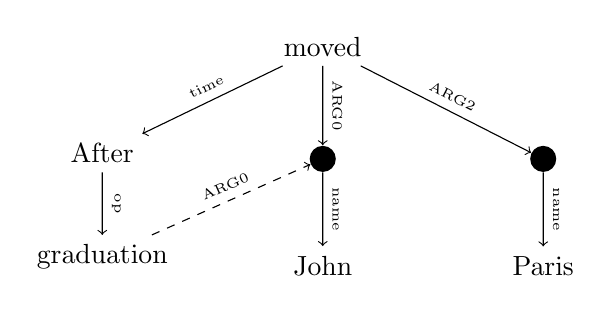
\begin{tikzpicture}[level distance=16mm, ->,
      every node/.append style={sloped,anchor=south,auto=false,font=\tiny},
      level 1/.style={sibling distance=28mm},
      level 2/.style={sibling distance=14mm},
      level 3/.style={sibling distance=12mm}]
    \tikzstyle{word} = [font=\rmfamily,color=black]
    \node (ROOT) [word] {moved}
      child {node [word] {After}
      {
            child {node (graduation) [word] {graduation} edge from parent node {op} }
      } edge from parent node {time} }
      child {node (John) [fill=black,circle] {}
      {
        child {node [word] {John} edge from parent node {name} }
      } edge from parent node {ARG0} }
      child {node [fill=black,circle] {}
      {
        child {node [word] {Paris} edge from parent node {name} }
      } edge from parent node {ARG2} }
      ;
      \draw[dashed] (graduation) to node {ARG0} (John);
  \end{tikzpicture}
  \captionof{figure}{Converted AMR graph, with
  text tokens added according to the alignments.
  Numeric suffixes of \textit{op} relations were removed,
  and names collapsed.}
  \label{fig:converted_example_amr}
\end{subfigure}

\begin{subfigure}{0.5\textwidth}
  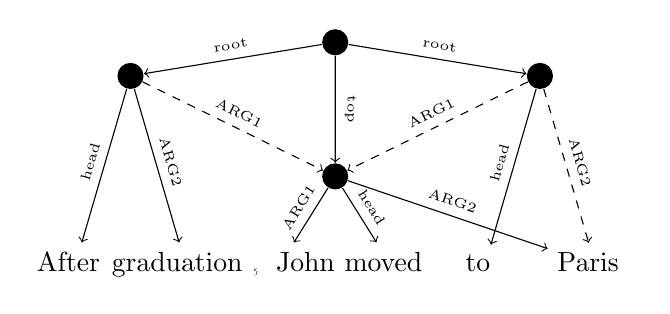
\begin{tikzpicture}[level distance=12mm, ->,
      every node/.append style={sloped,anchor=south,auto=false,font=\tiny},
      level 1/.style={sibling distance=26mm,level distance=6mm},
      level 2/.style={sibling distance=14mm,level distance=14mm}]
    \tikzstyle{word} = [font=\rmfamily,color=black]
    \node (ROOT) [fill=black,circle] {}
      child {node (after) [fill=black,circle] {}
      {
        child {node [draw=none] {}
        {
          child {node [word] (after_word) {After{\color{white}g}} edge from parent [draw=none]}
        } edge from parent [draw=none] }
        child {node [draw=none] {}
        {
          child {node [word] (graduation) {graduation ,} edge from parent [draw=none]}
        } edge from parent [draw=none] }
      } edge from parent node {root}}
      child {node [draw=none] {}
      {
        child {node (moved) [fill=black,circle] {}
        {
          child {node [word] {\quad{\color{white}g} John} edge from parent node {ARG1}}
          child {node [word] {moved{\color{white}g}} edge from parent node {head}}
        } edge from parent [draw=none] }
      } edge from parent [draw=none] }
      child {node (to) [fill=black,circle] {}
      {
        child {node [draw=none] {}
        {
            child {node [word] (to_word) {to{\color{white}g}} edge from parent [draw=none]}
          } edge from parent [draw=none] }
          child {node [draw=none] {}
        {
          child {node [word] (Paris) {Paris{\color{white}g}} edge from parent [draw=none]}
        } edge from parent [draw=none] }
      } edge from parent node {root}}
      ;
      \draw (ROOT) to node {top} (moved);
      \draw (after) to node {head} (after_word);
      \draw (after) to node {ARG2} (graduation);
      \draw[dashed] (after) to node {ARG1} (moved);
      \draw[dashed] (to) to node {ARG1} (moved);
      \draw (to) to node {head} (to_word);
      \draw (moved) to node {ARG2} (Paris);
      \draw[dashed] (to) to node {ARG2} (Paris);
  \end{tikzpicture}
  \captionof{figure}{Converted SDP graph (in the DM formalism), with
  intermediate non-terminal nodes introduced as \textit{head} units.
  In case of reentrancy, an arbitrary reentrant edge is marked as remote.}
  \label{fig:converted_example_sdp}
\end{subfigure}
~
\begin{subfigure}{0.5\textwidth}
  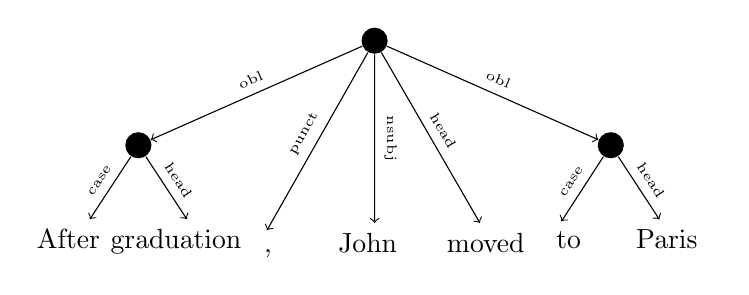
\begin{tikzpicture}[level distance=15mm, ->,
      every node/.append style={sloped,anchor=south,auto=false,font=\tiny},
      level 1/.style={sibling distance=15mm},
      level 2/.style={sibling distance=16mm}]
    \tikzstyle{word} = [font=\rmfamily,color=black]
    \node (ROOT) [fill=black,circle] {}
      child {node (after) [fill=black,circle] {}
      {
        child {node [word] {After{\color{white}g}} edge from parent node {case}}
        child {node [word] {graduation {\color{white}g}\quad\quad} edge from parent node {head}}
      } edge from parent node {obl}}
      child {node {}
      {
        child {node [word] (comma) {{\color{white}g} ,} edge from parent [draw=none]}
      } edge from parent [draw=none]}
      child {node {}
      {
        child {node [word] (John) {John{\color{white}g}} edge from parent [draw=none]}
      } edge from parent [draw=none]}
      child {node {}
      {
        child {node [word] (moved) {moved{\color{white}g}} edge from parent [draw=none]}
      } edge from parent [draw=none]}
      child {node (to) [fill=black,circle] {}
      {
          child {node [word] {\quad{\color{white}g}to} edge from parent node {case}}
          child {node [word] {Paris{\color{white}g}} edge from parent node {head}}
      } edge from parent node {obl}}
      ;
      \draw (ROOT) to node {punct} (comma);
      \draw (ROOT) to node {nsubj} (John);
      \draw (ROOT) to node {head} (moved);
  \end{tikzpicture}
  \captionof{figure}{Converted UD graph.
  As in SDP, intermediate non-terminals and \textit{head} edges are introduced.
  The graph is actually a tree, as was the original bilexical graph.}
  \label{fig:converted_example_ud}
\end{subfigure}

\caption{Unified DAG format
(pre-terminals omitted: each terminal drawn in place of its parent).}
\label{fig:converted_examples}
\end{figure*}


\section{Unified DAG format}\label{sec:conversion}

To be able to use TUPA for the four tasks presented in \S\ref{sec:tasks},
we convert them all into a unified DAG format.
In this format, the graph is a rooted DAG, and the text tokens are terminal nodes.
As in the UCCA format, the graph edges are labeled,
and are divided into \textit{primary} and \textit{remote} edges,
where the primary edges form a tree (all nodes have at most one primary parent,
and the root has none).
The remote edges enable reentrancy, and thus together with them the graph
is in general a DAG and not necessarily a tree.
Figure~\ref{fig:converted_examples} shows examples for converted graphs.
Converting UCCA into the unified format consists simply of removing linkage nodes
and edges (see Figure~\ref{fig:converted_example_ucca}).

\subsection{Converting bilexical dependencies}
To convert DM and UD into the unified DAG format,
we add a pre-terminal for each terminal,
and then attach the pre-terminals according to the original dependency edges.
We add an additional level with a \textit{head} edge to avoid terminal and non-terminal siblings
(see Figure~\ref{fig:converted_example_sdp} and Figure~\ref{fig:converted_example_ud}).
Since DM allows multiple roots, we attached the corresponding non-terminals as children of
the single converted graph root, with the \textit{root} edge label.
Top nodes are labeled with \textit{top} instead.
In case of reentrancy, an arbitrary parent is marked as primary, and the rest as remote
(denoted as dashed edges in Figure~\ref{fig:converted_examples}).

\subsection{Converting AMR}
In the conversion from AMR, non-terminals are already present and do not need to be introduced.
However, alignments and node labels must be handled
(see Figure~\ref{fig:converted_example_amr}).
Since alignment to the text tokens is not part of the AMR graph,
we introduce the alignments as edges in conversion.
We use automatically aligned AMR graphs provided in the dataset (see \S\ref{sec:data}),
and attach each node with a \textit{Terminal} edge to each of the terminals it is aligned to.

Since the order of AMR ordinal relations, such as \textit{op1}, \textit{op2},
is annotated according to the order of text tokens,
the numeric index is redundant and is thus removed.
We keep the numeric suffixes when they are meaningful, e.g. in \textit{ARG0}, \textit{ARG1}, etc.

Named entities in AMR are expressed by \textit{name} relations and nodes, with
a child for each token in the name, and relations labeled \textit{op1}, \textit{op2}, etc.
We instead collapse this subgraph to a single node whose children are the terminals
corresponding to the name tokens.


\begin{figure}[t]
   \begin{tikzpicture}
   \node[anchor=west] at (0,1.25) {Parser state};
   \draw[color=gray,dashed] (0,0) rectangle (7.5,1);
    \node (x4) at (3.75,0.5) {\ldots};
   \end{tikzpicture}
   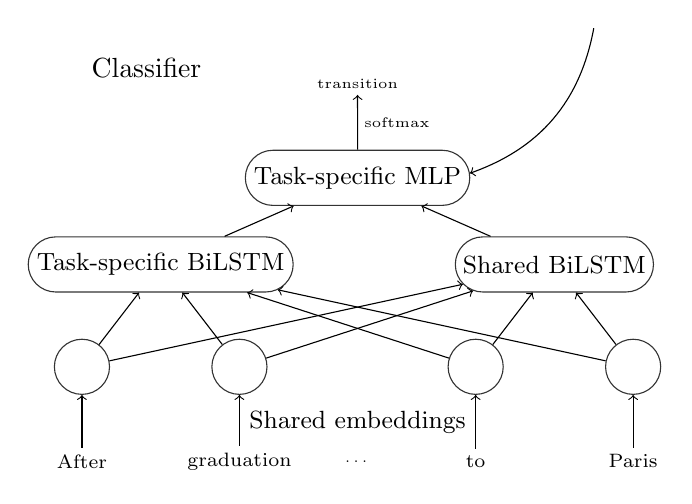
\begin{tikzpicture}[->]
   \node[anchor=west] at (0,6) {Classifier};
   \tiny
   \tikzstyle{main}=[rounded rectangle, minimum size=7mm, draw=black!80, node distance=12mm]
   \node[main] (specific) at (1,3.5) {\small Task-specific BiLSTM};
   \node[main] (shared) at (6,3.5) {\small Shared BiLSTM};
   \node (embeddings) at (3.5,1.5) {\small Shared embeddings};
   \foreach \i/\word in {0/{After},2/{graduation},5/{to},7/{Paris}} {
       \node (x\i) at (\i,1) {\scriptsize \word};
       \node[main] (e\i) at (\i,2.2) {};
       \path (x\i) edge (e\i);
       \path (e\i) edge (specific);
       \path (e\i) edge (shared);
   }
    \node (x4) at (3.5,1) {\ldots};
    \node[main] (mlp) at (3.5,4.6) {\small Task-specific MLP};
    \path (specific) edge (mlp);
    \path (shared) edge (mlp);
    \coordinate (state) at (6.5,6.5);
    \path (state) edge [bend left] (mlp);
    \node (transition) at (3.5,5.8) {transition};
    \path (mlp) edge node[right] {softmax} (transition);
   \end{tikzpicture}
   \caption{Multitask model.
      Representations for input tokens are computed by two BiLSTMs:
      a task-specific one and a share one. The result is concatenated with
      features from the parser state and fed into the MLP for selecting the next transition.}
   \label{fig:multi_model}
\end{figure}

\section{Multitask transition-based parsing}\label{sec:multitask}

Since the same TUPA model can be applied to different tasks, we can train it on multiple tasks together.
Rather than sharing all model parameters, we share only part of the model \cite{P17-1186}.
Feature embeddings are shared, and in addition to the task-specific BiLSTM,
we use a shared BiLSTM. The outputs of both BiLSTMs are concatenated and
fed into the task-specific MLP (see Figure~\ref{fig:multi_model}).

Multitask learning is particularly beneficial for improving on tasks with small training data.
As UCCA has a relatively small corpus (see \S\ref{sec:data}),
we focus on UCCA parsing and treat AMR, DM and UD parsing
as auxiliary tasks, creating a unified corpus by shuffling all sentences from all datasets together,
but using only the score on the UCCA development set as the criterion for early stopping.

\subsection{Unlabeled parsing for auxiliary tasks}\label{sec:unlabeled_aux}

The auxiliary tasks are quite difficult enough on their own.
Since it has been shown that easier auxiliary tasks are more beneficial
in multitask learning \cite{E17-2026},
we decided to use unlabeled parsing for all auxiliary tasks, while still doing
labeled UCCA parsing.


\section{Experiments}\label{sec:experiments}

We perform various experiments to evaluate the benefit of each auxiliary task to UCCA parsing.
First, we train the parser separately on each task.
Next, we train it to parser UCCA in a multitask setting, where AMR, DM and UD are used as
auxiliary tasks. Following previous work, we use the same hyperparameter settings
as for the single-task case \cite{N16-1179,P16-2038,C16-1013,C16-1059,C16-1179,E17-1005}.

\begin{table*}[ht]
\begin{tabular}{ll|rr|rr|rr}
\hline
& & \multicolumn{2}{c|}{English} & \multicolumn{2}{c|}{French} & \multicolumn{2}{c}{German} \\
\multicolumn{2}{c|}{Corpus} & {\#}tok & {\#}sent & {\#}tok & {\#}sent & {\#}tok & {\#}sent \\
\hline
\textbf{UCCA}
& Wiki & 158433 & 5225 &&&& \\
& 20K Leagues & 12339 & 506 & 12929 & 547 & 113524 & 4764 \\
\hline
\textbf{UD} & v2.1 & 568560 & 24276 & 540942 & 21567 & 318847 & 16590 \\
\hline
\textbf{AMR} & LDC2016E25 & 708701 & 39260 \\
\hline
\textbf{DM} & SemEval 2015 & 802717 & 35657 \\
\end{tabular}
\caption{Size of each corpus: total number of tokens ({\#}tok) and sentences
({\#}sent).\label{tab:corpora}}
\end{table*}

\subsection{Data}\label{sec:data}

For UCCA, we use the English Wikipedia corpus \cite{abend2013universal},
and the \textit{Twenty Thousand Leagues Under the Sea} corpus \cite[20K leagues;][]{sulem2015conceptual},
annotated in English, French and German.
For AMR, we use LDC2016E25, used in SemEval 2017 \cite{may2017semeval}.
For SDP, we use data for the DM target representation from SemEval 2015 \cite{oepen2015semeval}.
For Universal Dependencies, we use UD v2.1 \cite{11234/1-2515}.
Table~\ref{tab:corpora} shows the size of each corpus.

Since the UCCA corpus is disproportionally small in comparison to the auxiliary task corpora,
simply training on all training data would create a model that is geared toward the auxiliary tasks.
To overcome this problem,
at each training iteration we sample a subset of the training set for each auxiliary task.
The subset size is identical to the UCCA training set size.


\subsection{Evaluation}\label{sec:evaluation}

As each scheme has its own evaluation metric, we evaluate them separately.
For UCCA, we evaluate labeled precision, recall and F1 on primary and remote edges.
For UD, we use LAS F1.
For AMR, we use Smatch \cite{cai2013smatch}.
For DM, we use labeled precision, recall and F1.


\subsection{Results}\label{sec:results}




\subsection{Single-task parsing}\label{sec:results_single}

To evaluate the conversion and parsing algorithm on each task, we report the result
of training the parser on each task separately.
In this case we perform labeled parsing for all tasks, and use the whole training set.
The results for single-task parsing, when evaluated on the development set for each task,
are shown in Table~\ref{tab:single}.



\begin{table}
\begin{tabular}{l|ccc}
\textbf{UD English} && \multicolumn{2}{r}{\textbf{LAS F1}} \\
Ours &&& 80.1 \\
D\&M &&& 82.2 \\
\hline
\textbf{AMR} & \textbf{P} & \textbf{R} & \textbf{F1} \\
Ours & 66.7 & 64.7 & 65.7 \\
F\&M &&& 70.9 \\
\hline
\textbf{DM} & \textbf{LP} & \textbf{LR} & \textbf{LF} \\
Ours & 76 & 75.4 & 75.7 \\
CMU &&& 89.4
\end{tabular}
\caption{Single-task results on dev set for each auxiliary task,
when trained only on that task.
Best reported results given for comparison:
D\&M is \citet{dozat2016deep},
F\&M is \citet{foland2017abstract},
and CMU is \citet{thomson-EtAl:2014:SemEval}.
AMR is evaluated by Smatch \cite{cai2013smatch}.
\label{tab:single}}
\end{table}


\subsection{Multitask parsing}\label{sec:results_multi}

Next, we focus on UCCA parsing, and assess the contribution of each auxiliary task
and combinations thereof, by evaluating on the UCCA development set.
As mentioned in \S\ref{sec:unlabeled_aux}, we train on all auxiliary tasks as unlabeled tasks.
The results for multitask parsing are shown in Table~\ref{tab:multi}.

\begin{table}
\begin{tabular}{l|ccc|ccc}
\multirow{2}{1cm}{Aux. tasks} & \multicolumn{3}{c|}{Primary} & \multicolumn{3}{c}{Remote} \\
& \textbf{LP} & \textbf{LR} & \textbf{LF} & \textbf{LP} & \textbf{LR} & \textbf{LF} \\
\hline
TUPA & 74.5 & 74.9 & 74.7 & 49.2 & 50.5 & 49.8 \\
\hline
Single & 72.9 & 73 & 73 &53 & 47 & 49.8 \\
AMR & 73.1 & 73.4 & 73.3 & 44 & 50.5 & 47\\
UD & 73 & 73.4 & 73.2 & 48.3 & 51.7 & 49.9 \\
DM & 73.7 & 73.3 & 73.5 & 44 & 57.9 & 50 \\
\tiny DM+UD & 73.7 & 73.5 & 73.6 & 43.5 & 42.4 & 42.9 \\
\tiny AMR+UD & 73.5 & 73.4 & 73.4 & 51.3 & 42.4 & 46.4 \\
\tiny AMR+DM & 74.1 & 74.2 & 74.1 & 49.4 & 50.5 & 49.9 \\
All & 72.6 & 74.9 & 73.7 & 49.8 & 46.4 & 48.1
\end{tabular}
\caption{Results on UCCA Wiki dev set.
TUPA is from \citet{hershcovich2017a}\footnote{Our experiments
    reached slightly lower scores on primary edges}\label{tab:multi}}
\end{table}


\subsection{Other languages}\label{sec:multilingual}

To investigate the contribution of multitask training on an even smaller UCCA training set,
we experiment with the French and German \textit{20K Leagues} UCCA corpora
\cite{sulem2015conceptual}.
The results are given in Table~\ref{tab:multilingual}.
The contribution of multitask learning is substantial in this case:
although the classifier does not get even a single edge right on the tiny French dataset,
when coupled with UD parsing as an auxiliary task, it achieves high scores
in both languages.
This shows that a small UCCA training corpus may suffice, as long as it is complemented by
a large training corpus in an auxiliary task in the same language.

\begin{table}
\begin{tabular}{l|ccc|ccc}
& \multicolumn{3}{c|}{Primary} & \multicolumn{3}{c}{Remote} \\
& \textbf{LP} & \textbf{LR} & \textbf{LF} & \textbf{LP} & \textbf{LR} & \textbf{LF} \\
\multicolumn{4}{l|}{\textbf{German}} & \\
\multicolumn{4}{l|}{Single-task:} & \\
\small Ours & 54.2 & 38.4 & 45 & 35 & 17.3 & 23.1 \\
\multicolumn{4}{l|}{Multitask (UCCA + UD):} \\
\small Ours & 74.6 & 74.1 & 74.4 & 66 & 13.6 & 22.5 \\
\hline
\multicolumn{4}{l|}{\textbf{French}} & \\
\multicolumn{4}{l|}{Single-task:} & \\
\small Ours & -- & 0 & -- & -- & 0 & -- \\
\multicolumn{4}{l|}{Multitask (UCCA + UD):} & \\
\small Ours & 64.4 & 64.4 & 64.4 & 36.4 & 7.5 & 12.5
\end{tabular}
\caption{Single-task and multitask results on the UCCA 20K Leagues development set in German and French.\label{tab:multilingual}}
\end{table}



\section{Related work}\label{sec:related_work}

In general, multitask learning involves optimizing more than one loss function \cite{ruder2017overview}.
However, in our case, the loss function has the same form across all tasks.
The same architecture and inference algorithm are applied to multiple annotation formats and datasets,
and only some of the parameters are shared between them: this is hard parameter sharing.

Multitask learning is often used in NLP, both as regularization when little training data is available,
and as an alternative to the pipeline approach, to avoid error propagation
\cite{collobert2008unified}.
Multitask learning has been applied to semantic parsing, including
semantic dependency parsing \cite{P17-1186} and
frame semantic parsing \cite{swayamdipta2017frame}.
\citet{guo2016exploiting} applied multitask learning to transition-based
syntactic parsing,
both in a multilingual setting and with multiple formats in a single language.
In transition-based parsing, multitask learning has also been applied to
tagging and parsing \cite{bohnet2012transition,Zhang2016StackpropagationIR},
lexical and syntactic analysis \cite{constant-nivre:2016:P16-1,more2016joint},
and semantic-syntactic analysis \cite{swayamdipta-EtAl:2016:CoNLL,henderson2013multilingual}.


\section{Discussion}\label{sec:discussion}

\subsection{Common edges}\label{sec:common}

An important factor in the success of multitask learning is the commonalities between the tasks
\cite{E17-2026,E17-1005}.
In fact, this is why we decided to convert the auxiliary tasks into UCCA-like format for
multitask training in the first place.
To get a sense of the similarity between the converted formats and actual UCCA graphs,
we perform unlabeled evaluation of a sample annotated in each format, and gold-standard UCCA,
after conversion to the unified format.
The comparison is performed on 100 sentences from Section 00 of the Wall Street Journal
corpus, which were manually annotated in all four formats.\footnote{For UD, we converted the
data from Stanford Dependencies using Stanford CoreNLP, including enhanced and enhanced++
dependencies\cite{SCHUSTER16.779}}.
The results are listed in Table~\ref{tab:common}.

\begin{table}
\begin{tabular}{lccc|ccc}
& \multicolumn{3}{c|}{Primary} & \multicolumn{3}{c}{Remote} \\
& \textbf{UP} & \textbf{UR} & \textbf{UF} & \textbf{UP} & \textbf{UR} & \textbf{UF} \\
AMR & 52.2 & 15.5 & 23.9 & 7.3 & 5.5 & 6.3 \\
DM & 63.6 & 49.8 & 55.9 & 6.9 & 63.8 & 12.4 \\
UD & 75.3 & 82.9 & 78.9 & -- & 0 & -- \\
UD$^+$ & 75.1 & 82.4 & 78.5 & 11.5 & 12.8 & 12.1 \\
UD$^{++}$ & 75.1 & 82.5 & 78.6 & 11.8 & 12.8 & 12.2
\end{tabular}
\caption{Unlabeled UCCA evaluation of each scheme after conversion to the unified format.
UD$^+$ and UD$^{++}$ refer to the Enhanced and Enhanced++ Universal Dependencies,
respectively \cite{SCHUSTER16.779}.\label{tab:common}}
\end{table}


\bibliography{references}
\bibliographystyle{acl_natbib}

\end{document}
